 \subsubsection{assign\_values\_to\_qpoints.f90}

 \subsubsection{basis\_functions\_V.f90}
 This file contains 3 functions: 
 \subsubsection{compute\_dNdx\_dNdy\_dNdz.f90}
 This subroutine computes $\partial{\bN^\upnu}/\partial x$, $\partial{\bN^\upnu}/\partial y$ and
 $\partial{\bN^\upnu}/\partial z$ at a location $r,s,t$ passed as argument.
 \subsubsection{compute\_dNdx\_dNdy.f90}
 This subroutine computes $\partial{\bN^\upnu}/\partial x$ and $\partial{\bN^\upnu}/\partial y$
 at a location $r,s$ passed as argument.
 \subsubsection{compute\_elemental\_matrices.f90}
 Note that when the material model is called directly on the quadrature points and 
 the penalty formulation is used then the viscosity at the reduced quadrature location 
 is obtained by taking the maximum viscosity value carried by the quadrature points of 
 the element. 
 \subsubsection{compute\_elemental\_volumes}

 \subsubsection{impose\_boundary\_conditions}
 This subroutine modifies the elemental $\K$, $\G$ and $\C$ matrices as well as the 
 elemental rhs $f_{el}$ and $h_{el}$ and returns them modified after imposing
 velocity Dirichlet boundary conditions.
 \subsubsection{template}

 \subsubsection{interpolate\_onto\_nodes.f90}
 This subroutine interpolates the components of the strain rate tensor on the velocity nodes.
 \subsubsection{locate\_point}
 This file contains a few simple subroutines which deal with the localisation of a point 
 in the mesh. The {\tt locate\_point} subroutine receives the coordinates of a point as argument 
 and returns its reduced coordinates and the id of the element it sits in.
 It relies on 3 other subroutines ({\tt find\_ielx\_r}, {\tt find\_iely\_s}, {\tt find\_ielz\_t})
 which take as argument a coorinate (x,y,z) and return the corresponding reduced
 coordinate (r,s,t) and the integer coordinate (ielx,iely,ielz).
 \subsubsection{make\_matrix.f90}
 This subroutine loops over all elements, build their elemental matrices and rhs, 
 apply the boundary conditions ont these elemental matrices, and then 
 assembles them in the global matrix, either in CSR or in MUMPS format.
 \subsubsection{matrix\_setup\_GT.f90}

 \subsubsection{matrix\_setup\_K}

 \subsubsection{matrix\_setup\_M}
 See Section~\ref{ss:symmcsrss}. 
 \subsubsection{output\_mesh.f90}
 This subroutine produces the {\filenamefont meshV.vtu} file which only 
 contains the corner nodes.
 \subsubsection{output\_qpoints}

 \subsubsection{output\_solution}
 This subroutine generates the {\filenamefont solution.vtu} in the {\foldernamefont OUTPUT}
 folder. It also generates the basic ascii file {\filenamefont solution.ascii}
 \subsubsection{output\_swarm.f90}
 This subroutine produces the {\filenamefont swarm.vtu} file in the 
 {\foldernamefont OUTPUT} folder which contains the 
 swarm of particles with all their properties.
 \subsubsection{paint\_swarm}
 
 \subsubsection{pcg\_solver\_csr}
 The subroutine solves $A\cdot = b$ by means f the preconditioned Conjugate Gradient method
 and the implementation follows algorithm 2.2 on page 82 of Elman, Silvester \&
 Wathen \cite{elsw}:
 
 Choose ${\vec u}^{(0)}$, compute ${\vec \phi}^{(0)}={\bm A}\cdot {\vec u}^{(0)}$ 
 then ${\vec r}^{(0)}={\vec f}-{\vec \phi}^{(0)}$, 
 ${\vec z}^{(0)}={\bm M}^{-1}\cdot {\vec r}^{(0)}$ and set ${\vec p}^{(0)}={\vec z}^{(0)}$.
 
 For $k=0$ until convergence do
 \begin{itemize}
 \item ${\vec \phi}^{(k)}={\bm A}\cdot {\vec p}^{(k)}$
 \item compute $\alpha_k = <{\vec z}^{(k)},{\vec r}^{(k)}>/<{\vec \phi}^{(k)},{\vec p}^{(k)}>$
 \item ${\vec u}^{(k+1)}={\vec u}^{(k)}+\alpha_k {\vec p}^{(k)}$
 \item ${\vec r}^{(k+1)}={\vec r}^{(k)}-\alpha_k{\vec \phi}^{(k)}$
 \item test for convergence
 \item ${\vec z}^{(k+1)}=M^{-1} {\vec r}^{(k+1)}$
 \item $\beta_k= <{\vec z}^{(k+1)},{\vec r}^{(k+1)}>/<{\vec z}^{(k)},{\vec r}^{(k)}>$
 \item ${\vec p}^{(k+1)}={\vec z}^{(k+1)}+\beta_k {\vec p}^{(k)}$
 \end{itemize}
 The convergence test is $\| \vec{r}_{k+1} \|_2/ \| \vec{r}_{k+1} \|_2 < tol$, 
 the maximum number of iterations is set to 1000, and the relative tolerance to $tol=10^{-6}$.
 Since the preconditioned is the diagonal of the ${\bm A}$ matrix, then the inverse of 
 ${\bm M}$ is trivial to compute/apply. 
 \subsubsection{postprocessors.f90}
 This subroutine computes the root mean square velocity
 and each of the average velocity components. It also 
 computes the volume using GLQ.
 \subsubsection{prescribe\_stokes\_solution.f90}
 This subroutine prescribes the velocity, pressure, temperature and strain rate components
 on the corners of each element via the {\sl analytical\_solution} subroutine.
 \subsubsection{quadrature\_setup.f90}
 This subroutine allocates all GLQ-related arrays for each element.
 It further computes the real $(x_q,y_q,z_q)$ and reduced $(r_q,s_q,t_q)$
 coordinates of the GLQ points, and assigns them their weights.
 \subsubsection{recover\_pressure\_penalty}
 This is scheme 4 in Section~\ref{psmoothing} (see \stone~12) which was proven to be 
 very cheap and very accurate. 
 The viscosity at the reduced quadrature location 
 is obtained by taking the maximum viscosity value carried by the quadrature points of 
 the element. 
 \subsubsection{set\_default\_values}
 This subroutine assigns default values to many of the global variables.
 \subsubsection{set\_global\_parameters\_pair}

 \subsubsection{setup\_cartesian2D.f90}
 This subroutine assigns to every element the coordinates of the its velocity, pressure,
 and temperature nodes, the velocity, pressure and temperature connectivity arrays,
 the coordinates of its center (xc,yc), its integer coordinates (ielx, iely),
 and its dimensions (hx,hy).
 \begin{center}
 \begin{flushright} {\tiny {\color{gray} (tikz\_3x2\_q1.tex)}} \end{flushright}
%~~~~~~~~~~~~~~~~~~~~~~~~~~~~~~~~~~~~~~~~~~~~~~~~~~~~~~~~~~~~~~~~~~~~~~~~~~~~~~~~~~~~~~~~~~~~~~~~~~

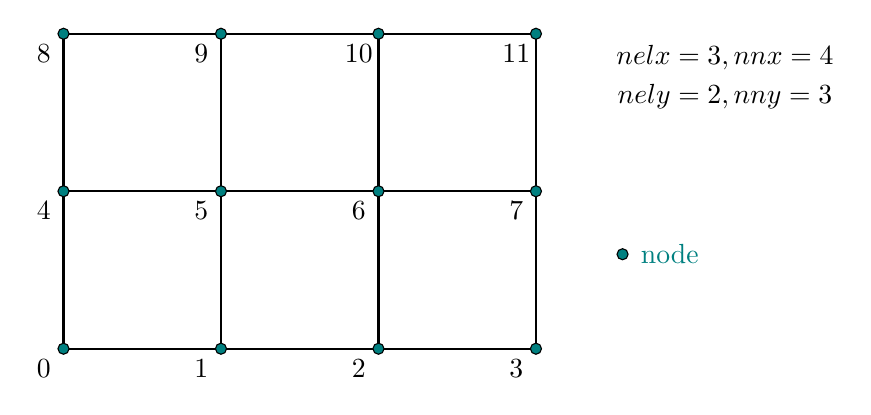
\begin{tikzpicture}
%\draw[step=0.5cm,gray,very thin] (0,0) grid (9,5); %background grid

\draw[thick] (1,1) -- (7,1) -- (7,5) -- (1,5) -- cycle;  
\draw[thick] (1,3) -- (7,3) ;
\draw[thick] (3,1) -- (3,5) ;
\draw[thick] (5,1) -- (5,5) ;

\draw[black,fill=teal] (1,1)     circle (2pt); 
\draw[black,fill=teal] (3,1)     circle (2pt); 
\draw[black,fill=teal] (5,1)     circle (2pt); 
\draw[black,fill=teal] (7,1)     circle (2pt); 

\draw[black,fill=teal] (1,3)     circle (2pt); 
\draw[black,fill=teal] (3,3)     circle (2pt); 
\draw[black,fill=teal] (5,3)     circle (2pt); 
\draw[black,fill=teal] (7,3)     circle (2pt); 

\draw[black,fill=teal] (1,5)     circle (2pt); 
\draw[black,fill=teal] (3,5)     circle (2pt); 
\draw[black,fill=teal] (5,5)     circle (2pt); 
\draw[black,fill=teal] (7,5)     circle (2pt); 

\node[] at (0.75,0.75) {0};
\node[] at (2.75,0.75) {1};
\node[] at (4.75,0.75) {2};
\node[] at (6.75,0.75) {3};

\node[] at (0.75,2.75) {4};
\node[] at (2.75,2.75) {5};
\node[] at (4.75,2.75) {6};
\node[] at (6.75,2.75) {7};

\node[] at (0.75,4.75) {8};
\node[] at (2.75,4.75) {9};
\node[] at (4.75,4.75) {10};
\node[] at (6.75,4.75) {11};

\draw[black,fill=teal] (8.1,2.2) circle (2pt); 
\node[] at (8.7,2.2) {{\color{teal}node}};

\node[] at (9.4,4.7) {$nelx=3, nnx=4$};
\node[] at (9.4,4.2) {$nely=2, nny=3$};

\end{tikzpicture}

 \end{center}
 \begin{verbatim}
 elt:  1  | iconV  1  2  6   5  iconP  1
 elt:  2  | iconV  2  3  7   6  iconP  2
 elt:  3  | iconV  3  4  8   7  iconP  3
 elt:  4  | iconV  5  6  10  9  iconP  4
 elt:  5  | iconV  6  7  11  10 iconP  5
 elt:  6  | iconV  7  8  12  11 iconP  6
 \end{verbatim}
 \begin{center}
 \begin{flushright} {\tiny {\color{gray} (tikz\_3x2\_mini.tex)}} \end{flushright}
%~~~~~~~~~~~~~~~~~~~~~~~~~~~~~~~~~~~~~~~~~~~~~~~~~~~~~~~~~~~~~~~~~~~~~~~~~~~~~~~~~~~~~~~~~~~~~~~~~~

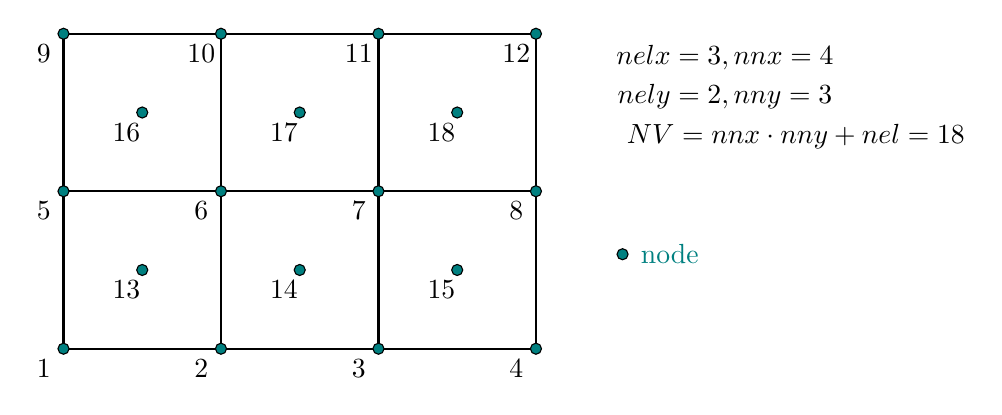
\begin{tikzpicture}
%\draw[step=0.5cm,gray,very thin] (0,0) grid (9,5); %background grid

\draw[thick] (1,1) -- (7,1) -- (7,5) -- (1,5) -- cycle;  
\draw[thick] (1,3) -- (7,3) ;
\draw[thick] (3,1) -- (3,5) ;
\draw[thick] (5,1) -- (5,5) ;

\draw[black,fill=teal] (1,1)     circle (2pt); 
\draw[black,fill=teal] (3,1)     circle (2pt); 
\draw[black,fill=teal] (5,1)     circle (2pt); 
\draw[black,fill=teal] (7,1)     circle (2pt); 

\draw[black,fill=teal] (1,3)     circle (2pt); 
\draw[black,fill=teal] (3,3)     circle (2pt); 
\draw[black,fill=teal] (5,3)     circle (2pt); 
\draw[black,fill=teal] (7,3)     circle (2pt); 

\draw[black,fill=teal] (1,5)     circle (2pt); 
\draw[black,fill=teal] (3,5)     circle (2pt); 
\draw[black,fill=teal] (5,5)     circle (2pt); 
\draw[black,fill=teal] (7,5)     circle (2pt); 

\draw[black,fill=teal] (2,2)     circle (2pt); 
\draw[black,fill=teal] (4,2)     circle (2pt); 
\draw[black,fill=teal] (6,2)     circle (2pt); 
\draw[black,fill=teal] (2,4)     circle (2pt); 
\draw[black,fill=teal] (4,4)     circle (2pt); 
\draw[black,fill=teal] (6,4)     circle (2pt); 

\node[] at (0.75,0.75) {1};
\node[] at (2.75,0.75) {2};
\node[] at (4.75,0.75) {3};
\node[] at (6.75,0.75) {4};

\node[] at (0.75,2.75) {5};
\node[] at (2.75,2.75) {6};
\node[] at (4.75,2.75) {7};
\node[] at (6.75,2.75) {8};

\node[] at (0.75,4.75) {9};
\node[] at (2.75,4.75) {10};
\node[] at (4.75,4.75) {11};
\node[] at (6.75,4.75) {12};

\node[] at (1.8,1.75) {13};
\node[] at (3.8,1.75) {14};
\node[] at (5.8,1.75) {15};
\node[] at (1.8,3.75) {16};
\node[] at (3.8,3.75) {17};
\node[] at (5.8,3.75) {18};

\draw[black,fill=teal] (8.1,2.2) circle (2pt); 
\node[] at (8.7,2.2) {{\color{teal}node}};

\node[] at (9.4,4.7) {$nelx=3, nnx=4$};
\node[] at (9.4,4.2) {$nely=2, nny=3$};
\node[] at (10.3,3.7) {$NV=nnx\cdot nny+nel=18$};

\end{tikzpicture}


 \end{center}
 \begin{verbatim}
 elt:  1  | iconV  1  2  6   5   13 iconP  1  2  6   5
 elt:  2  | iconV  2  3  7   6   14 iconP  2  3  7   6
 elt:  3  | iconV  3  4  8   7   15 iconP  3  4  8   7
 elt:  4  | iconV  5  6  10  9   16 iconP  5  6  10  9
 elt:  5  | iconV  6  7  11  10  17 iconP  6  7  11  10
 elt:  6  | iconV  7  8  12  11  18 iconP  7  8  12  11
 \end{verbatim}
 \begin{center}
 \begin{flushright} {\tiny {\color{gray} (tikz\_3x2\_q2.tex)}} \end{flushright}
%~~~~~~~~~~~~~~~~~~~~~~~~~~~~~~~~~~~~~~~~~~~~~~~~~~~~~~~~~~~~~~~~~~~~~~~~~~~~~~~~~~~~~~~~~~~~~~~~~~

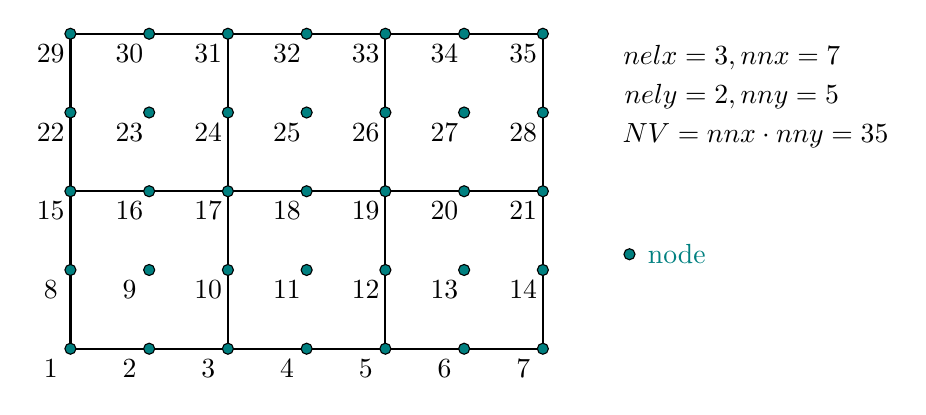
\begin{tikzpicture}
%\draw[step=0.5cm,gray,very thin] (0,0) grid (9,5); %background grid

\draw[thick] (1,1) -- (7,1) -- (7,5) -- (1,5) -- cycle;  
\draw[thick] (1,3) -- (7,3) ;
\draw[thick] (3,1) -- (3,5) ;
\draw[thick] (5,1) -- (5,5) ;

\draw[black,fill=teal] (1,1)     circle (2pt); 
\draw[black,fill=teal] (2,1)     circle (2pt); 
\draw[black,fill=teal] (3,1)     circle (2pt); 
\draw[black,fill=teal] (4,1)     circle (2pt); 
\draw[black,fill=teal] (5,1)     circle (2pt); 
\draw[black,fill=teal] (6,1)     circle (2pt); 
\draw[black,fill=teal] (7,1)     circle (2pt); 

\draw[black,fill=teal] (1,2)     circle (2pt); 
\draw[black,fill=teal] (2,2)     circle (2pt); 
\draw[black,fill=teal] (3,2)     circle (2pt); 
\draw[black,fill=teal] (4,2)     circle (2pt); 
\draw[black,fill=teal] (5,2)     circle (2pt); 
\draw[black,fill=teal] (6,2)     circle (2pt); 
\draw[black,fill=teal] (7,2)     circle (2pt); 

\draw[black,fill=teal] (1,3)     circle (2pt); 
\draw[black,fill=teal] (2,3)     circle (2pt); 
\draw[black,fill=teal] (3,3)     circle (2pt); 
\draw[black,fill=teal] (4,3)     circle (2pt); 
\draw[black,fill=teal] (5,3)     circle (2pt); 
\draw[black,fill=teal] (6,3)     circle (2pt); 
\draw[black,fill=teal] (7,3)     circle (2pt); 

\draw[black,fill=teal] (1,4)     circle (2pt); 
\draw[black,fill=teal] (2,4)     circle (2pt); 
\draw[black,fill=teal] (3,4)     circle (2pt); 
\draw[black,fill=teal] (4,4)     circle (2pt); 
\draw[black,fill=teal] (5,4)     circle (2pt); 
\draw[black,fill=teal] (6,4)     circle (2pt); 
\draw[black,fill=teal] (7,4)     circle (2pt); 

\draw[black,fill=teal] (1,5)     circle (2pt); 
\draw[black,fill=teal] (2,5)     circle (2pt); 
\draw[black,fill=teal] (3,5)     circle (2pt); 
\draw[black,fill=teal] (4,5)     circle (2pt); 
\draw[black,fill=teal] (5,5)     circle (2pt); 
\draw[black,fill=teal] (6,5)     circle (2pt); 
\draw[black,fill=teal] (7,5)     circle (2pt); 

\node[] at (0.75,0.75) {1};
\node[] at (1.75,0.75) {2};
\node[] at (2.75,0.75) {3};
\node[] at (3.75,0.75) {4};
\node[] at (4.75,0.75) {5};
\node[] at (5.75,0.75) {6};
\node[] at (6.75,0.75) {7};

\node[] at (0.75,1.75) {8};
\node[] at (1.75,1.75) {9};
\node[] at (2.75,1.75) {10};
\node[] at (3.75,1.75) {11};
\node[] at (4.75,1.75) {12};
\node[] at (5.75,1.75) {13};
\node[] at (6.75,1.75) {14};

\node[] at (0.75,2.75) {15};
\node[] at (1.75,2.75) {16};
\node[] at (2.75,2.75) {17};
\node[] at (3.75,2.75) {18};
\node[] at (4.75,2.75) {19};
\node[] at (5.75,2.75) {20};
\node[] at (6.75,2.75) {21};

\node[] at (0.75,3.75) {22};
\node[] at (1.75,3.75) {23};
\node[] at (2.75,3.75) {24};
\node[] at (3.75,3.75) {25};
\node[] at (4.75,3.75) {26};
\node[] at (5.75,3.75) {27};
\node[] at (6.75,3.75) {28};

\node[] at (0.75,4.75) {29};
\node[] at (1.75,4.75) {30};
\node[] at (2.75,4.75) {31};
\node[] at (3.75,4.75) {32};
\node[] at (4.75,4.75) {33};
\node[] at (5.75,4.75) {34};
\node[] at (6.75,4.75) {35};

\draw[black,fill=teal] (8.1,2.2) circle (2pt); 
\node[] at (8.7,2.2) {{\color{teal}node}};

\node[] at (9.4,4.7) {$nelx=3, nnx=7$};
\node[] at (9.4,4.2) {$nely=2, nny=5$};
\node[] at (9.7,3.7) {$NV=nnx\cdot nny=35$};

\end{tikzpicture}

 \end{center}
 \begin{verbatim}
 elt:  1  | iconV  1   2   3   8   9   10  15  16  17 iconP           1           2           6           5
 elt:  2  | iconV  3   4   5   10  11  12  17  18  19 iconP           2           3           7           6
 elt:  3  | iconV  5   6   7   12  13  14  19  20  21 iconP           3           4           8           7
 elt:  4  | iconV  15  16  17  22  23  24  29  30  31 iconP           5           6          10           9
 elt:  5  | iconV  17  18  19  24  25  26  31  32  33 iconP           6           7          11          10
 elt:  6  | iconV  19  20  21  26  27  28  33  34  35 iconP           7           8          12          11
 \end{verbatim}
 \subsubsection{setup\_cartesian3D.f90}
 This subroutine assigns to every element the coordinates of the its velocity, pressure,
 and temperature nodes, the velocity, pressure and temperature connectivity arrays,
 the coordinates of its center (xc,yc,zc), its integer coordinates (ielx,iely,ielz),
 and its dimensions (hx,hy,hz).
 \subsubsection{solve\_KVeqf}
 This subroutine solves the system $\K\cdot \vec{V} = \vec{f}$. The matrix is 
 implicit passed as argument via the module but the rhs and the guess vector are 
 passed as arguments.
 If MUMPS is used the system is solved via MUMPS (the guess is vector
 is then neglected), otherwise a call is made to  the {\tt solve\_cg\_diagprec} subroutine.
 \subsubsection{solve\_stokes}
 This subroutine solves the Stokes system: if it is a saddle point problem 
 it does so using the preconditioned conjugate gradient (PCG) applied 
 to the Schur complement $\SSS$  (see Section~\ref{ss:schurpcg}).
 If the penalty method is used 
 \subsubsection{spmv\_kernels}
 This file contains the Sparse Matrix-Vector multiplication kernels (see Section~\ref{ss:spmv}).
 \subsubsection{swarm\_setup.f90}
 This subroutine generates the swarm of particles. The layout is controled 
 by the {\tt init\_marker\_random} parameter.
 \begin{center}
 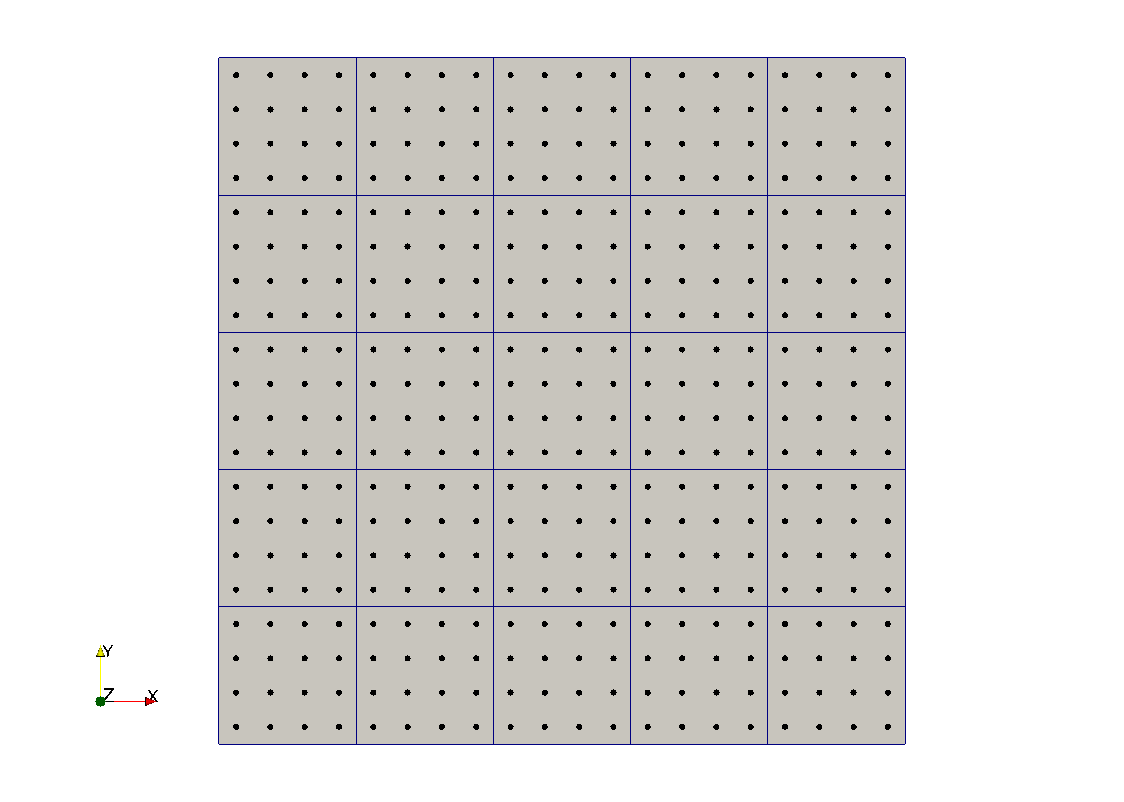
\includegraphics[width=5cm]{ELEFANT/images/swarm_reg} 
 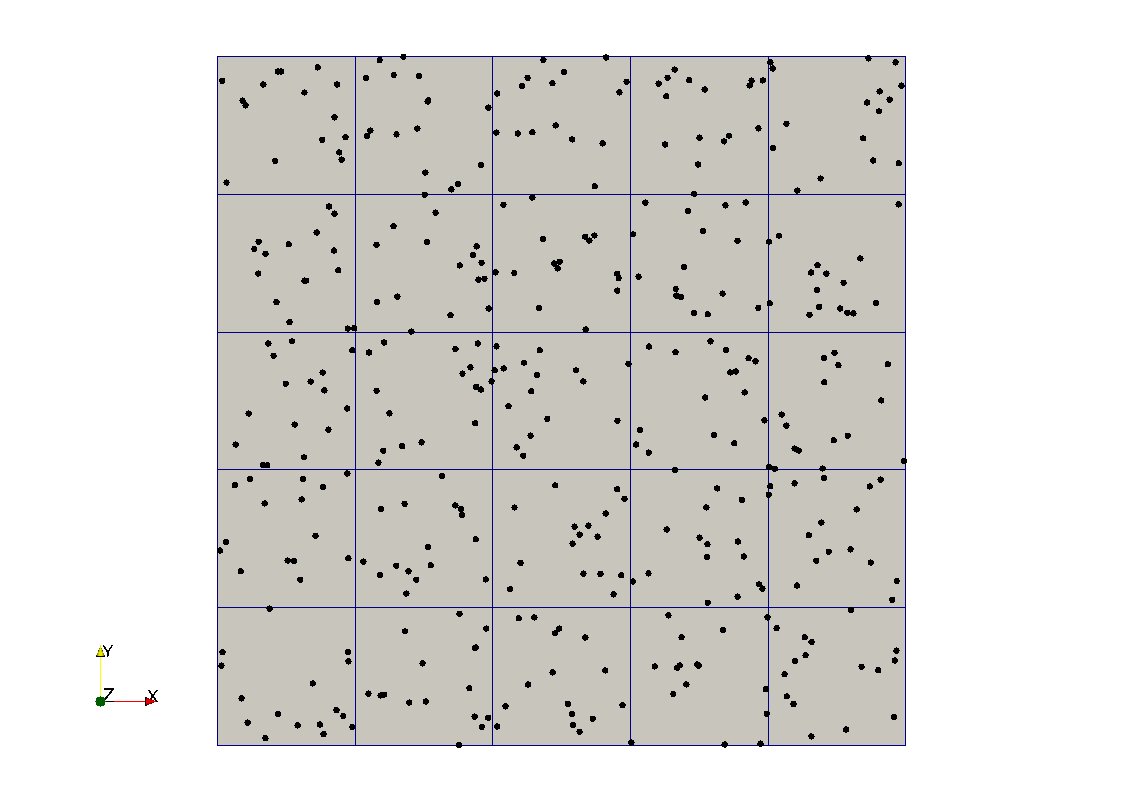
\includegraphics[width=5cm]{ELEFANT/images/swarm_rand} 
 \end{center}
 \subsubsection{template}

 \subsubsection{test\_basis\_functions}
 This subroutine tests the consistency of the basis functions. 
 An analytical velocity field is prescribed (constant, linear or quadratic) and the 
 corresponding values are computed onto the quadrature points via the 
 (derivatives of the) basis functions.
 It generates three ascii files in the {\foldernamefont OUTPUT} folder which 
 are to be processed with the gnuplot script present there.
 \subsubsection{write\_stats}

